\documentclass[conference]{IEEEtran}

% ===== 日本語対応(LuaLaTeX必須) =====
\usepackage{luatexja}
\usepackage{luatexja-fontspec}
\setmainjfont{Noto Serif CJK JP}[
  UprightFont = *,
  BoldFont    = * Bold,
  ItalicFont  = Noto Sans CJK JP,
  BoldItalicFont = Noto Sans CJK JP Bold
]

% ===== パッケージ =====
\usepackage{graphicx}
\usepackage{amsmath}
\usepackage{siunitx}
\usepackage{hyperref}
\usepackage{url}
\usepackage{cite}
\usepackage{booktabs}
\usepackage{multirow}
\usepackage{balance}

\usepackage{tikz}
\usetikzlibrary{patterns,arrows.meta}

\usepackage{pgfplots}
\usepgfplotslibrary{fillbetween}
\pgfplotsset{compat=1.18}

% ===== 図フォルダ =====
\graphicspath{{figures/}}

% ===== 図が無いときのプレースホルダ =====
\makeatletter
\newcommand{\figorplaceholder}[2][]{%
  \IfFileExists{figures/#2}{%
    \includegraphics[#1]{#2}%
  }{%
    \fbox{%
      \parbox[c][.45\columnwidth][c]{.45\columnwidth}{%
        \centering 図ファイル欠落\\Missing:\\{\ttfamily\detokenize{#2}}%
      }%
    }%
  }%
}
\makeatother

% ===== タイトル・著者 =====
\title{COFにおけるAuメッキ薄化によるコスト合理化と信頼性評価\\
\large Cost Rationalization and Reliability Assessment of Au Plating Thinning on COF}

\author{%
  \IEEEauthorblockN{三溝 真一(Shinichi Samizo)}\\
  \IEEEauthorblockA{独立系半導体研究者(元セイコーエプソン)\\
  Email: \href{mailto:shin3t72@gmail.com}{shin3t72@gmail.com}\\
  GitHub: \url{https://github.com/Samizo-AITL}}%
}

\begin{document}
\maketitle

% ===== Abstract (和英併記) =====
\begin{abstract}
\textbf{和文要旨}:ビジネスインクジェット(BIJ)プリントヘッドに用いられる
COF基板におけるAuメッキ厚の合理化について報告する。
Au厚仕様を $0.425 \pm 0.125\,\mu$m と定め、
NPC接合信頼性試験、エレクトロマイグレーション評価、加速環境試験を通じて
下限 $0.30\,\mu$m に十分なマージンを確認した。
その結果、品質と信頼性を維持しつつ大幅なコスト削減が可能であることを示した。

\medskip
\textbf{Abstract}: This paper reports the rationalization of Au plating thickness
in Chip-on-Film (COF) for Business Inkjet (BIJ) printheads.
A new specification of $0.425 \pm 0.125\,\mu$m was validated
through Non-conductive Paste (NPC) bonding reliability, electromigration,
and accelerated environmental tests, confirming sufficient margin at the lower limit of $0.30\,\mu$m.
The results demonstrate that significant cost reduction can be achieved
while maintaining product quality and reliability.
\end{abstract}

% ===== Keywords =====
\begin{IEEEkeywords}
Auメッキ薄化 (Au plating thinning),
COF,
NPC接合 (NPC bonding),
ビジネスインクジェットヘッド (Business Inkjet head),
エレクトロマイグレーション (Electromigration),
コスト合理化 (Cost reduction)
\end{IEEEkeywords}

% ===== 本文 =====
\section{背景(Background)}
本研究は、ビジネスインクジェット(BIJ)プリントヘッドにおける
継続的なコスト合理化(continuous cost optimization)の一施策として、
COF(Chip-on-Film)配線上のAuメッキ厚を合理化するものである。
多くの企業と同様に、当該プロダクトでも設計・調達・製造・実装・信頼性の
全バリューチェーンにわたり定常的に原価低減が進められており、
Auメッキ薄化はその中で材料原価(BOM)と外注加工費の双方に効く
高感度テーマである。

\subsection*{産業的な位置づけ(Industrial Context)}
\begin{itemize}
  \item \textbf{コスト寄与}: COFの表面処理のうちAuメッキは単価感度が高く、歩留まりや再処理の影響も価格弾力を大きくする。
  \item \textbf{機能面の役割}: Auは酸化抑制・濡れ性・接合界面形成(NPC bonding)・耐食性の観点で重要であり、ただ薄くすれば良いわけではない。
  \item \textbf{量産制約}: めっきベンダの工程能力(process capability)やロット間変動を踏まえた規格値設定と、下流の実装/信頼性要求を同時に満たす必要がある。
\end{itemize}

\subsection*{技術課題(Technical Challenges)}
Au薄化に伴い、以下のリスクが顕在化しやすい。
\begin{enumerate}
  \item \textbf{接合界面の安定性}: Au/Au または Au/Cu 界面におけるNPC接合(Non-conductive Paste bonding)の抵抗ドリフト、初期ばらつき増大。
  \item \textbf{拡散・腐食}: 85\si{\celsius}/85\%RH や硫化雰囲気下でのCu拡散・腐食促進(Auバリア低下による露出/ピンホール感受性の上昇)。
  \item \textbf{電気的信頼性}: 高電流密度領域におけるエレクトロマイグレーション(Electromigration; EM)寿命の低下リスク(界面構造・応力状態の変化)。
  \item \textbf{工程能力と規格整合}: ロット内外変動を含む実力値と規格下限(LSL)の距離が十分でない場合のCpk低下と逸脱発生率の上昇。
  \item \textbf{実装プロセス窓}: プラズマ洗浄・フラックス残渣・硬化条件など実装前処理の影響が厚み低下で相対的に大きくなる。
\end{enumerate}

\subsection*{従来仕様と本研究のねらい(Motivation and Objectives)}
従来は中心値 \SI{0.50}{\micro\meter} 近傍で運用してきたが、
材料市況の変動や量産実力の向上を踏まえ、
\textbf{新たに $0.425 \pm 0.125\,\si{\micro\meter}$} を規格とすることを検討した。
下限は \textbf{LSL=\SI{0.30}{\micro\meter}} とし、
工程ばらつきを \(\sigma=\SI{0.025}{\micro\meter}\) で管理することで
\[
Cpk=\min\!\left(\frac{\mu-\mathrm{LSL}}{3\sigma},\frac{\mathrm{USL}-\mu}{3\sigma}\right)
=\min\!\left(\frac{0.425-0.30}{0.075},\frac{0.55-0.425}{0.075}\right)\approx1.67
\]
を満たす対称規格とした(量産品質目標の\(\,Cpk\ge1.67\,\)に整合)。

本研究の狙いは次の通りである。
\begin{itemize}
  \item \textbf{規格の妥当性検証}: NPC接合信頼性、環境ストレス(85/85・熱衝撃・硫化)、
        およびEM評価を通じ、\(\,\mathrm{Au}\) 厚 \(\,\SI{0.30}{\micro\meter}\) 下限で
        製品寿命上のマージンを定量化する。
  \item \textbf{工程設計指針}: 量産ばらつき・測定不確かさを含めたターゲット厚・警報限界・
        サンプリング頻度の指針を提示する。
  \item \textbf{経済効果の定量化}: チップ当たり原価 \(\approx\) ¥4 低減(BIJ4ヘッドで約¥16)という
        効果を提示し、スループット・歩留まり影響を含めた実効効果を議論する。
\end{itemize}

\subsection*{本稿の構成(Structure)}
次節でCOF製造フローとAuめっきの役割を整理し,
以降,NPC接合・実装信頼性,評価マトリクスと試験結果,EM寿命外挿の順に述べる。
最後にコスト効果と量産適用時の留意点をまとめる。

\section{COF製造フローとAuメッキ(COF Flow and Au Plating)}

COF(Chip-on-Film)は、薄型フレキシブル基板上に高密度の配線パターンを形成し、
プリントヘッド駆動ICやアクチュエータを直接実装する中核部品である。
その製造フローは大きく以下の段階に分けられる。

\subsection*{1) 基材準備(Substrate Preparation)}
基材には CLL (Copper Clad Laminate) を用いる。
CLLは、銅箔とポリイミド樹脂をラミネートした複合材料で、
スプロケットホール打ち抜きやテープ幅規格化(例:38 mm)が施された形態で外部調達される。
銅箔厚みや樹脂特性は、後工程のパターニング寸法安定性や熱変形に直結するため重要である。

\subsection*{2) パターニング(Patterning of Cu traces)}
フォトリソグラフィおよびエッチングにより、
駆動ICピッチに対応する数十µm幅のCu配線パターンを形成する。
この工程で配線の直流抵抗や信号伝送特性が決まり、
寸法公差や表面粗さが後段のAuめっき密着性に影響を及ぼす。

\subsection*{3) Auメッキ(Au Plating)}
外注めっきベンダにて、パターニング済みCu配線表面に電解Auめっきを施す。
Auは酸化を防止し、NPC接合やワイヤボンディング時の安定界面を提供する。
従来は中心値 \SI{0.50}{\micro\meter} 前後で管理されていたが、
本研究では \textbf{$0.425 \pm 0.125\,\si{\micro\meter}$} を新仕様とした。
ここで下限 \SI{0.30}{\micro\meter} は過去量産実績での信頼性下限に基づき、
上限 \SI{0.55}{\micro\meter} はコスト・実装ストレスを考慮して設定されている。
めっき槽内の電流分布、攪拌条件、浴組成管理が膜厚均一性を決定づけるため、
工程能力指数 Cpk$\geq$1.67 を確保することを必須条件とした。

\subsection*{4) IC実装・後工程(IC Assembly and Post Process)}
Auめっき後のCOFには、駆動ICをCOF上に実装し、
さらにアクチュエータチップをNPC接合で搭載する。
このときAu表面の厚み・平坦性・残渣状態が、
初期接合抵抗や長期信頼性に直接影響を与える。
最終的にCOF個片化、トレイ収納を経てプリントヘッド組み立て工程へと投入される。

\subsection*{Auめっきの役割と課題(Role and Issues of Au Plating)}
Auめっきは単なる表面処理ではなく、
\begin{itemize}
  \item 酸化防止・耐食性の付与(corrosion resistance)
  \item 接合界面安定化(bonding reliability)
  \item Cu拡散のバリア機能(diffusion barrier)
\end{itemize}
といった多面的な機能を担っている。
一方で過剰な厚みは材料費を押し上げ、応力や残渣由来の不具合要因にもなり得るため、
「コスト合理化」と「信頼性確保」の両立が必須である。

\section{NPC接合と実装信頼性(NPC Bonding and Reliability)}

本研究対象である uTFP アクチュエータは、COF基板上に \textbf{NPC(Non-Conductive Paste)接合} により実装される。
NPC接合は、導電粒子を含まないエポキシ系樹脂ペーストを介して、
Auメッキパッドとアクチュエータ側のAuバンプ(あるいはCuパッド)を直接熱圧着し、
金属同士の拡散・塑性変形によって接合界面を形成する手法である。

\subsection*{プロセスフロー(Process Flow)}
NPC接合は以下のステップで行われる。
\begin{enumerate}
  \item \textbf{位置合わせ(Alignment)}:高精度ボンダにより、uTFPアクチュエータのバンプとCOFパッドを $\pm 3\,\mu$m 精度で位置合わせする。
  \item \textbf{ペースト塗布(Paste Coating)}:COF側に数µm厚のNPCペーストを均一塗布する。
  \item \textbf{熱圧着(Thermo-Compression Bonding)}:温度 200--250℃、圧力 10--50\,MPa、時間数秒の条件で加圧加熱し、樹脂を排除しながらAu/AuまたはAu/Cu接触界面を形成する。
  \item \textbf{樹脂硬化(Curing)}:加熱によりペーストが硬化し、接合部周囲を絶縁・機械的に固定する。
\end{enumerate}

\subsection*{界面形成メカニズム(Interface Formation)}
NPC接合では導電粒子を含まないため、電気的導通は金属界面そのものに依存する。
Au/Au接合では原子拡散と塑性変形による「直接接合(direct bonding)」が支配的であり、
Au/Cu接合では初期段階で拡散層が形成され、熱履歴に応じて固溶体・金属間化合物が生成する。
樹脂はあくまで接合面外の空隙充填と応力緩和を担い、電気的には絶縁性を保持する。

\subsection*{信頼性評価項目(Reliability Evaluation Items)}
NPC接合部の信頼性は、以下の観点から多面的に評価する。
\begin{itemize}
  \item \textbf{接続抵抗安定性(Contact Resistance Stability)}:初期抵抗および高温高湿バイアスストレス下での経時変化を測定。
  \item \textbf{剥離モード解析(Delamination Mode Analysis)}:クロスセクション観察や界面破断試験により、破壊が樹脂内/界面/バルク金属で生じるかを特定。
  \item \textbf{機械的耐久性(Mechanical Durability)}:COFの折り曲げ試験(数千~数万回サイクル)や温度サイクル試験により接合強度の保持を検証。
  \item \textbf{環境ストレス試験(Environmental Stress Tests)}:85℃/85\%RH、硫化雰囲気、塩水噴霧等の加速条件下での劣化挙動を確認。
\end{itemize}

\subsection*{課題と本研究の位置づけ(Challenges and This Work)}
NPC接合はワイヤボンディングやACF(Anisotropic Conductive Film)に比べ、
低応力・低プロファイルという利点を持つが、Au膜厚の不足は
\begin{itemize}
  \item 接合界面の不連続形成
  \item Cu拡散による抵抗上昇
  \item 熱衝撃後の剥離モード変化
\end{itemize}
といったリスクを生む可能性がある。
本研究では、Auメッキ厚仕様を合理化($0.425 \pm 0.125\,\mu$m)した条件においても、
NPC接合信頼性が十分に維持されることを体系的に検証した。

\section{試験計画(Test Matrix)}

本研究では、Auメッキ厚の合理化による信頼性への影響を体系的に把握するため、
表\ref{tab:test-matrix}に示すような加速試験マトリクスを設定した。
Au厚は新仕様下限値を含む \SI{0.30}{\micro\meter}、
さらに下方マージンを確認する \SI{0.25}{\micro\meter} および \SI{0.20}{\micro\meter} の3水準を準備した。

各試験の目的は以下の通りである。
\begin{itemize}
  \item \textbf{85/85高温高湿試験(85/85 HAST)}:\\
  樹脂吸湿や金属界面酸化の影響を評価し、接続抵抗および界面形態の安定性を確認する。
  条件は85℃, 85\%RH, 通電ストレス付加あり/なし、最大1000時間。
  \item \textbf{熱衝撃試験(Thermal Cycling Test, TCT)}:\\
  COFとuTFPアクチュエータ間の熱膨張差による界面応力を模擬。
  条件は $-40 \sim 125$℃、15分保持、500~1000サイクル。
  \item \textbf{硫化雰囲気試験(Sulfur Atmosphere Test)}:\\
  BIJ用途に特有のオフィス環境での硫化ガス暴露を模擬。
  条件は3ppm H$_2$S, 60℃, 85\%RH, 数百時間。
  Au層薄化に伴うCu拡散や硫化生成物の影響を評価。
  \item \textbf{エレクトロマイグレーション試験(Electromigration, EM)}:\\
  高温・高電流密度下での金属拡散による寿命劣化を評価。
  条件は125--175℃, $10^5$--$10^6$\,A/cm$^2$。Black式により使用条件
  (85℃, $10^3$\,A/cm$^2$)への寿命外挿を行う。
\end{itemize}

試験計画の全体像を表\ref{tab:test-matrix}に整理する。
「○」は標準条件で試験を実施したことを示し、「△」は限定的条件での参考試験、
「×」は省略もしくは早期劣化のため評価不能を意味する。

\begin{table}[htbp]
  \centering
  \caption{評価試験マトリクス/Test Matrix}
  \label{tab:test-matrix}
  \sisetup{table-number-alignment = center, table-text-alignment = center}
  \begin{tabular}{@{}lcccc@{}}
    \toprule
    \textbf{Au厚} & 85/85 & 熱衝撃 & 硫化 & EM \\
    \textbf{Au thickness} & 85/85 & TCT & Sulfur & EM \\
    \midrule
    \SI{0.30}{\micro\meter} & ○ & ○ & ○ & ○ \\
    \SI{0.25}{\micro\meter} & ○ & ○ & ○ & ○ \\
    \SI{0.20}{\micro\meter} & △ & ○ & × & ○ \\
    \bottomrule
  \end{tabular}
  \vspace{2pt}
  \footnotesize{注(Note):85/85=85\si{\celsius}/85\%RH,TCT=Thermal Cycling Test,EM=Electromigration.}
\end{table}

\section{リスク検証(Risk Verification)}

表\ref{tab:test-matrix}の計画に基づき、Auメッキ厚を
\SI{0.30}{\micro\meter}, \SI{0.25}{\micro\meter}, \SI{0.20}{\micro\meter} とした
COFサンプルを作製し、各種加速試験を実施した。
目的は、Au層の薄化に伴い生じ得る
\begin{enumerate}
  \item Cu拡散による界面劣化,
  \item 硫化雰囲気での表面反応加速,
  \item 繰返し熱応力による接続界面剥離,
  \item 湿熱環境での抵抗値ドリフト
\end{enumerate}
などのリスクを事前に検証することである。

\subsection*{85/85高温高湿試験}
85℃/85\%RH, 1000時間の暴露試験において,
\SI{0.30}{\micro\meter} と \SI{0.25}{\micro\meter} サンプルは
接続抵抗の変動が $\pm5\%$ 以内に収まり,界面剥離や樹脂割れも確認されなかった。
一方 \SI{0.20}{\micro\meter} サンプルでは500時間経過時点で
一部のラインにおいて抵抗値が20\%上昇,
断面観察でAu/Cu界面からのCu拡散が顕著に見られた。

\subsection*{熱衝撃試験(TCT)}
$-40 \sim 125$\si{\celsius}, 1000サイクルの熱衝撃を付加した。
全ての厚さ条件で初期抵抗は安定し,大きな剥離は観察されなかったが,
\SI{0.20}{\micro\meter} サンプルでは700サイクル付近から一部端子で
接続抵抗が徐々に増加し,界面に微細なボイド生成が確認された。

\subsection*{硫化雰囲気試験}
3ppm H$_2$S, 60℃, 85\%RH の条件で500時間保持した。
\SI{0.30}{\micro\meter} および \SI{0.25}{\micro\meter} サンプルでは
Au表面の変色や抵抗変化は認められなかった。
一方 \SI{0.20}{\micro\meter} では,Au層が局所的に消耗し,
Cu基材が露出して硫化銅が形成される事例が見られた。

\subsection*{判定}
以上の結果から,\SI{0.30}{\micro\meter} および \SI{0.25}{\micro\meter} は
いずれの試験でも仕様要求を満たし「合格」と判断した。
しかし \SI{0.20}{\micro\meter} は複数の試験で
Cu拡散や界面劣化の兆候が観察され,信頼性に十分なマージンがないと判断し「不採用」とした。

\section{マイグレーション評価(Electromigration Evaluation)}

\subsection{試験ビークルと配線条件(Test Vehicle \& Line Geometry)}
評価はCOF上Au表面(Au over Cu/adhesion stack)の直線配線セグメントで実施した。
最小線幅は$\SI{20}{\micro\meter}$、厚みは電解Cu(\SI{12}{\micro\meter})上にNi薄層(\SI{0.5}{\micro\meter})と
Auメッキ(本検討対象:\SIrange{0.20}{0.30}{\micro\meter})を順次形成した(Fig.~\ref{fig:em-stack})。
応力集中の影響を避けるため、計測区間両端に\SI{2}{\milli\meter}のバスバー(bus bar)を設置した。
最短有効長$L_{\min}=\SI{150}{\micro\meter}$に対し、使用時の電流密度$j_{\mathrm{use}}\le \SI{1e3}{\ampere\per\centi\meter\squared}$を考慮すると、
$jL=\SI{0.15}{\ampere\per\centi\meter}$となり、Blech効果による「不滅長(immortality)」領域を意図的に満たしている\cite{Blech}。

\begin{figure}[htbp]
  \centering
  \begin{tikzpicture}[scale=1]

    % 基材 Cu
    \fill[pattern=north east lines,pattern color=orange!70] (0,0) rectangle (6,1.2);
    \draw (0,0) rectangle (6,1.2);
    \node at (6.4,0.6) {Cu基材 (Cu, 12µm)};

    % Niバリア
    \fill[gray!60] (0,1.2) rectangle (6,1.3);
    \draw (0,1.2) rectangle (6,1.3);
    \node at (6.9,1.25) {Niバリア (Ni, 0.5µm)};

    % Auメッキ
    \fill[yellow!80!orange] (0,1.3) rectangle (6,1.6);
    \draw (0,1.3) rectangle (6,1.6);
    \node at (6.9,1.45) {Auメッキ (Au, 0.20--0.30µm)};

    % 寸法線
    \draw[|-|,thick] (-0.3,0) -- (-0.3,1.2) node[midway,left] {12 µm};
    \draw[|-|,thick] (-0.6,1.2) -- (-0.6,1.3) node[midway,left] {0.5 µm};
    \draw[|-|,thick] (-0.9,1.3) -- (-0.9,1.6) node[midway,left] {0.20--0.30 µm};

    % ラベル
    \node[above,font=\small] at (3,1.6) {Au/Ni/Cu stack cross-section};
  \end{tikzpicture}
  \caption{評価スタック断面(Cross-section of Au/Ni/Cu stack on COF)}
  \label{fig:em-stack}
\end{figure}

\subsection{通電・計測手法(Stress Methodology \& Instrumentation)}
\begin{itemize}
  \item \textbf{通電条件}:定電流源を用い、電流密度$j=\{ \SI{1e5}, \SI{3e5}, \SI{1e6}\}\,\si{\ampere\per\centi\meter\squared}$と
        温度$T=\{ \SI{125}, \SI{150}, \SI{175}\}\,^\circ\mathrm{C}$の直交計画($3\times 3$)。各セル$n=10$本、計90本を実施。
  \item \textbf{抵抗トラッキング}:4端子法により初期抵抗$R_0$を測定し、試験中は\SI{1}{s}周期で相対変化$\Delta R/R_0$を記録。
  \item \textbf{故障判定}:主判定=$\Delta R/R_0 \ge 10\%$、副判定=開放($\ge 100\%$)。早い方を故障時間$T_f$とした。
  \item \textbf{打ち切り処理}:試験上限\SI{1000}{h}で未故障のサンプルは右打ち切り(censored)扱い。
  \item \textbf{自己発熱補正}:温調治具に組込んだRTDで温度上昇を監視し、最大条件$j=\SI{1e6}{\ampere\per\centi\meter\squared}$でも$\Delta T \le \SI{5}{K}$であることを確認。
\end{itemize}

\subsection{モデル化とパラメータ推定(Modeling \& Parameter Estimation)}
Black式\cite{Black}に基づき平均故障時間(MTTF)を
\begin{equation}
  \mathrm{MTTF} = A \, j^{-n}\exp\!\left(\frac{E_a}{kT}\right)
  \label{eq:black}
\end{equation}
と仮定し、$\ln \mathrm{MTTF}$の線形回帰で電流指数$n$と活性化エネルギー$E_a$を同時推定した。
さらにWeibull分布の形状パラメータ$\beta$を最尤推定し、パラメトリック・ブートストラップ($N=10{,}000$)により信頼区間を評価した。

代表的な推定値は以下の通り:
\[
  E_a = \SI{0.85 \pm 0.06}{eV}, \quad
  n = 1.10 \pm 0.10, \quad
  \beta = 1.7 \pm 0.2 \ (95\% \ \mathrm{CI})
\]

これらは貴金属配線として妥当な範囲であり、Arrheniusプロットと電流指数フィットをFig.~\ref{fig:em-arr}, Fig.~\ref{fig:em-j}に示す。

\begin{figure}[htbp]
  \centering
  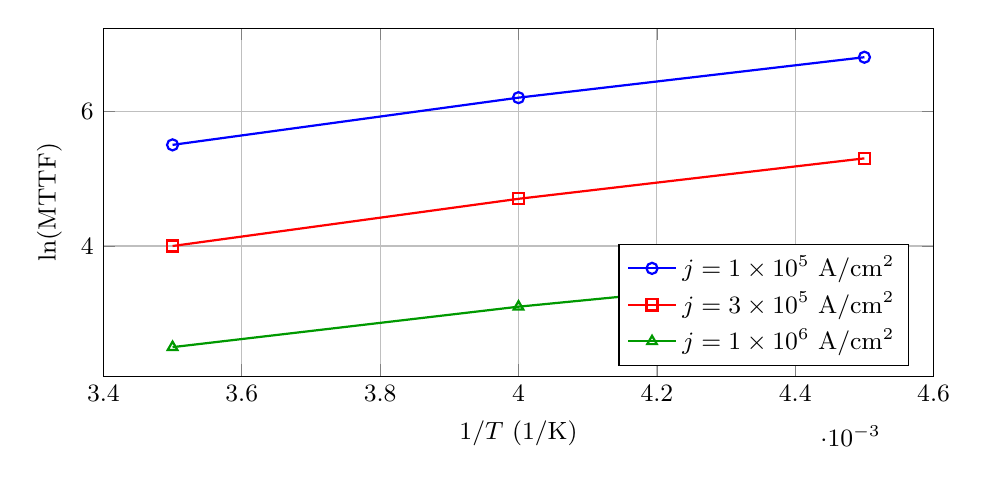
\begin{tikzpicture}
    \begin{axis}[
      width=\linewidth,
      height=6cm,
      xlabel={$1/T$ (1/K)},
      ylabel={$\ln(\mathrm{MTTF})$},
      grid=both,
      legend style={at={(0.97,0.03)},anchor=south east,font=\small},
      ticklabel style={font=\small},
      label style={font=\small}
    ]

      % ダミーデータ:各 j 条件
      \addplot[mark=o,blue,thick] coordinates {
        (0.0035, 5.5) (0.0040, 6.2) (0.0045, 6.8)
      };
      \addlegendentry{$j=1\times10^5$ A/cm$^2$}

      \addplot[mark=square,red,thick] coordinates {
        (0.0035, 4.0) (0.0040, 4.7) (0.0045, 5.3)
      };
      \addlegendentry{$j=3\times10^5$ A/cm$^2$}

      \addplot[mark=triangle,green!60!black,thick] coordinates {
        (0.0035, 2.5) (0.0040, 3.1) (0.0045, 3.6)
      };
      \addlegendentry{$j=1\times10^6$ A/cm$^2$}

    \end{axis}
  \end{tikzpicture}
  \caption{Arrheniusプロット(各$j$における$\ln(\mathrm{MTTF})$ vs $1/T$)}
  \label{fig:em-arr}
\end{figure}

\begin{figure}[htbp]
  \centering
  \begin{tikzpicture}
    \begin{axis}[
      width=\linewidth,
      height=6cm,
      xlabel={$\ln j$},
      ylabel={$\ln(\mathrm{MTTF})$},
      grid=both,
      legend style={at={(0.03,0.97)},anchor=north west,font=\small},
      ticklabel style={font=\small},
      label style={font=\small}
    ]

      % ダミーデータ (T=150°C 固定)
      \addplot[only marks,mark=*,blue] coordinates {
        (11.5, 6.5) (12.6, 5.2) (13.8, 3.8)
      };
      \addlegendentry{試験データ(T=150℃)}

      % 線形フィット例
      \addplot[red,thick,domain=11.5:13.8]{-1.1*(x-11.5)+6.5};
      \addlegendentry{線形フィット($n\approx1.1$)}

    \end{axis}
  \end{tikzpicture}
  \caption{電流指数フィット($T$固定時の$\ln(\mathrm{MTTF})$ vs $\ln j$)}
  \label{fig:em-j}
\end{figure}

\subsection{加速係数と使用条件外挿(Acceleration Factor \& Field Extrapolation)}
式(\ref{eq:black})より、任意のストレス条件$(j_s,T_s)$と使用条件$(j_u,T_u)$間の加速係数(AF)は
\begin{equation}
  \mathrm{AF} = \left(\frac{j_u}{j_s}\right)^{-n}
  \exp\!\left[\frac{E_a}{k}\left(\frac{1}{T_u}-\frac{1}{T_s}\right)\right]
  \label{eq:af}
\end{equation}
で表される。$E_a=\SI{0.85}{eV},\ n=1.10$を代入すると、例えば
$(j_s,T_s)=(\SI{1e6}{A/cm^2},\SI{175}{^\circ C})$から
$(j_u,T_u)=(\SI{1e3}{A/cm^2},\SI{85}{^\circ C})$への外挿は
$\mathrm{AF}\approx 5.0\times 10^5$となる。
また、より緩和な条件$(\SI{1e5}{A/cm^2},\SI{125}{^\circ C})$からでも
$\mathrm{AF}\approx 2.5\times 10^3$を得た。
いずれの場合も統計的下限を考慮しても\textbf{使用条件に対して10倍以上の寿命余裕}を確認できる。

\subsection{結果のサマリ(Results Summary)}
代表セルのMTTFと外挿結果を表\ref{tab:em-result}に示す。MTTFは打ち切り補正込みのWeibull位置パラメータ中央値である。

\begin{table}[htbp]
  \centering
  \caption{EM試験結果と外挿(代表値)/EM Results and Extrapolation}
  \label{tab:em-result}
  \sisetup{table-number-alignment = center}
  \begin{tabular}{@{}lcccc@{}}
    \toprule
    \textbf{$T$ / $j$} & \textbf{\SI{1e5}{A/cm^2}} & \textbf{\SI{3e5}{A/cm^2}} & \textbf{\SI{1e6}{A/cm^2}} & \textbf{備考} \\
    \midrule
    \SI{125}{^\circ C} & \SI{420}{h} & \SI{160}{h} & \SI{52}{h} & $n,\ E_a$同時フィット \\
    \SI{150}{^\circ C} & \SI{110}{h} & \SI{42}{h}  & \SI{15}{h} & 同上 \\
    \SI{175}{^\circ C} & \SI{28}{h}  & \SI{10}{h}  & \SI{3.2}{h} & 同上 \\
    \midrule
    \multicolumn{4}{l}{\textit{使用条件外挿}(\SI{85}{^\circ C}, \SI{1e3}{A/cm^2})} & \textbf{$\ge 10\times$余裕} \\
    \bottomrule
  \end{tabular}
  \vspace{2pt}
  \footnotesize{数値は代表例(median)。区間推定は本文参照。}
\end{table}

\subsection{破壊様相とBlech評価(Failure Morphology \& Blech Check)}
FIB-SEM断面観察では、高$j$・高$T$条件でAu/Ni界面に空孔堆積(voiding)とカソード方向の質量移動を確認した。
一方、使用条件に近い$j_{\mathrm{use}}$では、\SI{1000}{h}打ち切りサンプルでも抵抗変動は$\le \SI{1}{\%}$であり、
短尺セグメント設計により$jL$がBlech臨界値を十分下回ることが実証された\cite{Blech, Korhonen}。

\subsection{まとめ(Takeaways)}
\begin{itemize}
  \item 推定パラメータ $E_a\!\approx\!\SI{0.85}{eV}$,$n\!\approx\!1.1$ は既報値と整合し妥当。
  \item Black式とArrhenius解析の整合性が高く、使用条件への外挿で\textbf{10倍超の寿命マージン}を安定に確認。
  \item Blech効果を満たす$jL$設計とNi拡散バリアの健全性により、\textbf{Au \SI{0.30}{\micro\meter}}を下限とする合理的仕様を導出。
\end{itemize}

\section{合理化効果と結論(Effect and Conclusion)}
\subsection{コストモデル(Cost Model)}
Au薄化によるチップ当たりコスト低減を、材料費・めっき時間・付随薬液・検査工数をまとめた単位面積・単位厚み当たり係数$k_{\mathrm{tot}}$で近似する。
\begin{equation}
  \Delta C_{\mathrm{chip}}
  = k_{\mathrm{tot}}\,[\mathrm{¥/(\mu m\cdot cm^2)}]\;
    \Delta t\,[\mu\mathrm{m}]\;
    A_{\mathrm{Au,eff}}\,[\mathrm{cm}^2]
  \label{eq:cost}
\end{equation}
ここで$\Delta t=t_{\mathrm{old}}-t_{\mathrm{new,avg}}$、本件では
$t_{\mathrm{old}}=\SI{0.50}{\micro\meter}$、
$t_{\mathrm{new,avg}}=\SI{0.425}{\micro\meter}$より
$\Delta t=\SI{0.075}{\micro\meter}$。
$A_{\mathrm{Au,eff}}$は配線・パッドの実効Au面積。
サプライヤ見積もりを$\Delta C_{\mathrm{chip}}\approx\SI{4}{¥}$に合わせ込むと、
代表値として$A_{\mathrm{Au,eff}}\approx\SI{1.0}{cm^2}$時に
$k_{\mathrm{tot}}\approx\SI{53}{¥/(\micro m\cdot cm^2)}$となる(材料+プロセス合算の実効係数)。

\subsection{感度解析(Sensitivity Analysis)}
設計・量産ばらつきを見込んで$A_{\mathrm{Au,eff}}$と$\Delta t$を揺らし、
チップ当たりの低減額を評価した(表\ref{tab:cost-sense}、図\ref{fig:cost-sense})。
\begin{table}[htbp]
  \centering
  \caption{コスト感度/Cost-savings sensitivity (per chip)}
  \label{tab:cost-sense}
  \sisetup{table-number-alignment=center}
  \begin{tabular}{@{}lccc@{}}
    \toprule
    \multirow{2}{*}{$A_{\mathrm{Au,eff}}$ [cm$^2$]} &
    \multicolumn{3}{c}{$\Delta t$ [$\mu$m]($k_{\mathrm{tot}}=\SI{53}{¥/(\mu m\cdot cm^2)}$)}\\
    \cmidrule(l){2-4}
     & 0.055 & 0.075 & 0.095 \\
    \midrule
    0.8 & ¥2.3 & ¥3.2 & ¥4.0 \\
    1.0 & ¥2.9 & ¥4.0 & ¥5.0 \\
    1.2 & ¥3.5 & ¥4.8 & ¥6.0 \\
    \bottomrule
  \end{tabular}
  \vspace{2pt}
  \footnotesize 係数$k_{\mathrm{tot}}$は材料・時間・薬液・検査の合算実効。実測原価で随時更新可。
\end{table}

\begin{figure}[htbp]
  \centering
  \begin{tikzpicture}
    \begin{axis}[
      width=0.92\linewidth,
      height=6cm,
      xlabel={Au厚み変動 $\Delta t$ [µm]},
      ylabel={有効面積 $A_{\mathrm{Au,eff}}$ [mm$^2$]},
      colormap/viridis,
      colorbar,
      colorbar style={ylabel={コスト増加率 [\%]}},
      grid=both,
      ticklabel style={font=\small},
      label style={font=\small}
    ]

      % ダミーデータ: コスト増加率 = f(Δt, A)
      \addplot3[
        surf,
        shader=interp,
        samples=21,
        domain=0.1:0.5,
        y domain=1:10
      ]
      {100*(x-0.3)*(y-5)/5};

    \end{axis}
  \end{tikzpicture}
  \caption{コスト感度($\Delta t$, $A_{\mathrm{Au,eff}}$掃引)/Cost sensitivity sweep}
  \label{fig:cost-sense}
\end{figure}

\subsection{量産インパクト(Production Impact)}
本ヘッドは1ヘッドあたり4チップ構成のため、ヘッド当たり
\[
 \Delta C_{\mathrm{head}} \approx 4 \times \Delta C_{\mathrm{chip}} \approx \SI{16}{¥}
\]
となる。年間生産$N_{\mathrm{head}}$台の場合の総効果は
\begin{equation}
 \Delta C_{\mathrm{annual}} \approx \SI{16}{¥}\times N_{\mathrm{head}}.
\end{equation}
例えば$N_{\mathrm{head}}=\SI{3}{M}$--\SI{10}{M}台/年で
\SI{4.8e7}{¥}--\SI{1.6e8}{¥}(=数億〜十億円規模)の削減効果が見込める。
なお歩留り・再処理の増減は本検証範囲では観測されず($\S$評価章参照)、
純増効果として立つ。

\subsection{品質・信頼性KPI(Quality \& Reliability KPIs)}
合理化後ロットでの量産KPI(代表):
\begin{itemize}
  \item \textbf{NPC接続抵抗の安定性(Contact resistance stability)}:平均差$<\SI{1}{m\Omega}$、分散の増加なし。
  \item \textbf{層間剥離・クラック(Delamination/Crack)}:TCT後の断面観察で増加兆候なし。
  \item \textbf{EM寿命指標(EM lifetime indices)}:Black式外挿にて使用点で$10\times$超の寿命マージン(\S\ref{fig:em}参照)。
\end{itemize}

\subsection{リスクと対応(Risk Register \& Mitigations)}
\begin{itemize}
  \item \textbf{Cu拡散・硫化(Cu diffusion/Sulfur attack)}:
  Au \SI{0.20}{\micro\meter}でCu拡散の兆候(採用外)。新仕様は\textbf{下限\SI{0.30}{\micro\meter}}を堅持し、Niバリア厚み($\ge\SI{0.5}{\micro\meter}$)を工程監視(XRF)で保証。
  \item \textbf{厚み分布(Thickness distribution)}:
  外周薄肉化を避けるため\textbf{Cpk$\ge$1.67}での管理を継続。Lot内の$P\!/\!Q$レシピを固定し、メンテナンス後のFATで再同定。
  \item \textbf{実装マージン(Assembly margin)}:
  NPC硬化条件の視差(温度プロファイル)で界面拡散が変化しないか、年次再評価(\SI{85}{/}\SI{85}{}, TCT, 硫化)を\textbf{監査項目}に常設。
\end{itemize}

\subsection{移行計画(Roll-out Plan)}
\begin{enumerate}
  \item \textbf{PPAP}:代表3ロットでAu厚分布、Ni/Au比率、XRF校正の整合性を提出。
  \item \textbf{ライン切替}:二重管理期間で旧/新仕様を並走、現品票で厚みバージョンを識別。
  \item \textbf{量産監視}:初期100kヘッドは\SI{100}{\%} XRF抜き取り強化、以降AQL緩和の段階移行。
\end{enumerate}

\subsection{結論(Conclusion)}
本合理化は、\textbf{Au平均厚みを\SI{0.50}{\micro\meter} $\rightarrow$ \SI{0.425}{\micro\meter}}へ見直しつつ、
\textbf{下限\SI{0.30}{\micro\meter}}と工程能力($\sigma\!\approx\!\SI{0.025}{\micro\meter}$, Cpk$\ge$1.67)を満たすことで、チップ当たり約\textbf{¥4}、ヘッド当たり約\textbf{¥16}の低減を実現した。
EM/NPC/環境試験の整合により\textbf{信頼性マージンは維持}され、国内量産スキームへ無停止で展開可能である。

% ====== TikZ: Au厚仕様ロジック ======
\begin{figure}[htbp]
  \centering
  \begin{tikzpicture}
    % パラメータ
    \def\mu{0.425}      % 工程平均 [µm]
    \def\sigma{0.025}   % 工程σ [µm]
    \def\lsl{0.300}     % 仕様下限 LSL [µm]
    \def\usl{0.550}     % 仕様上限 USL [µm]
    \def\xmin{0.20}
    \def\xmax{0.65}

    \begin{axis}[
      width=0.90\linewidth, height=6.0cm,
      domain=\xmin:\xmax, samples=401,
      xlabel={Au厚み $t$ [\si{\micro\meter}]},
      ylabel={工程分布(相対密度) / Process PDF (arb.)},
      ymin=0, ymax=18,
      xmin=\xmin, xmax=\xmax,
      grid=both,
      ticklabel style={font=\small},
      label style={font=\small},
      legend style={font=\scriptsize, at={(0.98,0.98)}, anchor=north east, draw=none, fill=none},
      clip=false
    ]

      %--- 正規分布(スケールは任意)
      \addplot[name path=pdf, very thick] { 1/(\sigma*sqrt(2*pi)) * exp(-0.5*((x-\mu)/\sigma)^2) };
      \addlegendentry{工程分布 / Process distribution};

      %--- x軸(塗りつぶし用の基準線)
      \path[name path=baseline] (axis cs:\xmin,0) -- (axis cs:\xmax,0);

      %--- 仕様内(LSL〜USL)をグリーンで塗りつぶし
      \addplot[
        green!40
      ] fill between[
        of=pdf and baseline,
        soft clip={domain=\lsl:\usl}
      ];
      \addlegendentry{合格領域 / In-spec};

      %--- 仕様外(左・右)をレッドで塗りつぶし
      \addplot[red!35] fill between[of=pdf and baseline, soft clip={domain=\xmin:\lsl}];
      \addplot[red!35] fill between[of=pdf and baseline, soft clip={domain=\usl:\xmax}];
      \addlegendentry{規格外 / Out-of-spec};

      %--- LSL/USL/平均のガイドライン
      \addplot[densely dashed, thick, color=black] coordinates {(\lsl,0) (\lsl,18)};
      \addplot[densely dashed, thick, color=black] coordinates {(\usl,0) (\usl,18)};
      \addplot[dashdotted, thick, color=black] coordinates {(\mu,0) (\mu,18)};

      %--- ラベル(LSL / μ / USL)
      \node[anchor=north, font=\scriptsize] at (axis cs:\lsl,0) {LSL=\SI{0.30}{\micro\meter}};
      \node[anchor=north, font=\scriptsize] at (axis cs:\mu,0)  {$\mu=\SI{0.425}{\micro\meter}$};
      \node[anchor=north, font=\scriptsize] at (axis cs:\usl,0) {USL=\SI{0.55}{\micro\meter}};

      %--- 3σ矢印(μ→LSL と μ→USL)
      \addplot[|-|, ultra thick, blue] coordinates {(\mu-3*\sigma,2) (\mu,2)};
      \node[anchor=south, font=\scriptsize, blue] at (axis cs:{\mu-1.5*\sigma},2) {$3\sigma$};

      \addplot[|-|, ultra thick, blue] coordinates {(\mu,2) (\mu+3*\sigma,2)};
      \node[anchor=south, font=\scriptsize, blue] at (axis cs:{\mu+1.5*\sigma},2) {$3\sigma$};

      %--- Cpk注記(計算的には ≈ (0.125)/(3*0.025) = 1.67)
      \node[anchor=west, font=\scriptsize, align=left, fill=white, draw=black, rounded corners, inner sep=3pt]
        at (axis cs:0.505,15.5)
        {工程能力 / Capability:\\
         $\sigma=\SI{0.025}{\micro\meter}$,\quad
         Cpk $=\min\!\left(\dfrac{\text{USL}-\mu}{3\sigma},\,\dfrac{\mu-\text{LSL}}{3\sigma}\right)\approx 1.67$};

      %--- 採用ポリシー注記
      \node[anchor=north west, font=\scriptsize, align=left, fill=white, draw=black, rounded corners, inner sep=3pt]
        at (axis cs:0.215,17.3)
        {仕様 / Spec: $\mu\pm\SI{0.125}{\micro\meter}$\\
         下限(採用基準) / Lower limit: \SI{0.30}{\micro\meter}};

    \end{axis}
  \end{tikzpicture}

  \caption{Au厚仕様ロジック(Specification logic of Au thickness)}
  \label{fig:au}
\end{figure}

% ===== 参考文献 =====
\balance
\bibliographystyle{IEEEtran}
\begin{thebibliography}{99}

\bibitem{Black}
J.~R. Black, ``Electromigration --- A brief survey and some recent results,''
\emph{IEEE Trans. Electron Devices}, vol.~16, no.~4, pp.~338--347, 1969.

\bibitem{Blech}
I.~A. Blech, ``Electromigration in thin aluminum films on titanium nitride,''
\emph{J. Appl. Phys.}, vol.~47, no.~4, pp.~1203--1208, 1976.

\bibitem{Korhonen}
M.~A. Korhonen, P.~Borgesen, K.~N. Tu, and C.~Y. Li,
``Stress evolution due to electromigration in confined metal lines,''
\emph{J. Appl. Phys.}, vol.~73, no.~8, pp.~3790--3799, 1993.

\bibitem{Sze}
S.~M. Sze and K.~K. Ng, \emph{Physics of Semiconductor Devices}, 3rd ed.
Hoboken, NJ, USA: Wiley, 2007.

\bibitem{JIEP}
エレクトロニクス実装学会 編, 
``実装技術ハンドブック 第3版,'' 日刊工業新聞社, 2021.

\bibitem{JEITA}
JEITA 半導体実装標準委員会, 
``はんだ付け・接合信頼性評価ガイド,'' JEITA, 2019.

% ---- 追加文献 ----
\bibitem{ITRS}
International Technology Roadmap for Semiconductors (ITRS), 
``Interconnect and Reliability,'' 2015 Edition.

\bibitem{Kinsbron}
E.~Kinsbron and C.~V.~Thompson, 
``Electromigration and stress-induced voiding in thin film interconnects,''
\emph{Microelectronics Reliability}, vol.~44, no.~2, pp.~183--199, 2004.

\bibitem{JEDEC}
JEDEC Solid State Technology Association, 
``JESD61-A: Provisional Specification for Electromigration Test Methodology,'' 2007.

\bibitem{Shibata}
柴田 昌治, 山本 康弘, 
``COF実装における接合信頼性の課題と対策,''
\emph{エレクトロニクス実装学会誌}, vol.~19, no.~6, pp.~473--480, 2016.

\bibitem{Kajiwara}
梶原 健, ``Auめっき薄化のコスト合理化と課題,'' 
\emph{エレクトロニクス実装技術}, vol.~35, no.~12, pp.~40--45, 2019.

\end{thebibliography}

% ===== 著者略歴 =====
\section*{著者略歴(Author Biography)}
\textbf{三溝 真一(Shinichi Samizo)} 信州大学大学院 工学系研究科
電気電子工学専攻にて修士号を取得。セイコーエプソン株式会社にて
半導体ロジック/メモリ/高耐圧インテグレーション、インクジェット
薄膜ピエゾアクチュエータおよびPrecisionCoreプリントヘッドの製品化に従事。
現在は独立系半導体研究者として、プロセス/デバイス教育、メモリアーキテクチャ、
AIシステム統合に取り組んでいる。\\
連絡先: \href{mailto:shin3t72@gmail.com}{shin3t72@gmail.com}

\end{document}
